\section{Results}
%\subsection{Model consistency}
%To assess the model accuracy, we first simulate data using different parameter values, find the MLEs for the parameters from the simulated data, and then investigate the accuracy of the estimates by looking at the mean squared error and confidence intervals.\\

We analyzed two sets of nucleotide data, one is of yeast species and the other of the insects. 

\subsection{Results on Rokas et al.'s data on yeast}
We analyzed data previously studied by \citet{rokas2003nature}.
This genome sequence data have been obtained for 7 {\it Saccharomyces} species ({\it S. cerevisiae, S. paradoxus, S. mikatae, S. kudriavzevii, S. bayanus, S.castellii} and {\it S. kluyveri}) as well as for the outgroup fungus {\it Candida albicans}.
It includes 106 genes that are distributed throughout the {\it S. cerevisiae} genome on all 16 chromomosomes and comprises a total length of 42,342 amino acids.
\citet{rokas2003nature} analyzed this data set to investigate the conflict of gene trees.
We use the tree topology that is supported by the concatenated genome sequence, which is also supported by the majority of the genes as found by \citet{rokas2003nature}.
Since the new model is not time reversible the tree is rooted at the out group {\it C.alb}.\\

\subsubsection{maximum likelihood estimation}
First, the 106 gene sequences are concatenated as 1 whole sequence with 42,342 amino acids.
We use ProtTest \citep{prottest, Guindon2003phyml} to find maximum log-likelihood values under empirical models and compare their AIC values.
We also find the maximum log likelihood values under our new model, with all 3 approaches to determine the optimal amino acids.
In all the analyses, tree branch lengths are optimized while the topology is fixed. \\

\noindent The log-likelihood values and the AIC values are compared in Table \ref{table:mle}.\\
%Under the empirical models, the substitution rates are fixed instead of being optimized. 
%$I$ denotes that proportion of invariable sites is estimated in the model, $G$ means that Gamma distributed rate variation across all sites is included in the model.
%In models with $F$, amino acid frequencies are treated as free parameters and estimated by the observed frequencies in the sequence data.
%Otherwise, the equilibrium frequencies under the substitution rate matrix are used.\\

\noindent Under the new model, amino acid frequencies are the observed frequencies in the sequences therefore counted as 19 free parameters.
In addition, there are 5 free parameters for exchange rates between nucleotides with the rate between G and T fixed as 1, 14 branch lengths for the 8-species rooted phylogeney, Grantham sensitivity $g$, 2 free parameters for the weights in the physicochemical distance formula $\beta$ and $\gamma$. These 41 parameters are optimized in the maximum likelihood analyses as well as the optimal amino acids.\\

\begin{table}[h]
\begin{center}
\begin{tabular}{l r c r r}
\hline
Model & $\Delta$AIC & $l$ & Tree length & Parameters \\
\hline
New+maj & 0.00 & -257790.10 &  10.43 & 41 \\
New+max & 48574.60 & -239735.40 & 11.73 & 42,383 \\
New+weights & 123688.60 & -319615.40 & 2.86 & 60 \\
LG+I+G+F & 81803.98 & -298699.09 &  & 34\\
LG+G+F & 81808.86 & -298702.53 & & 33 \\
\hline
\end{tabular}
\end{center}
\caption{Log-likelihood values and parameter estimates under empirical models and new model for the sequence with 42,342 amino acids}
\label{table:mle}
\end{table}
%%notes on weighted approach when different genes use different weights
{\color{blue} Note: The last two models in the table are the best models picked out by ProtTest.(What happens when the weights of amino acids being optimal are gene specific and other parameters are fixed across genes? Total number of parameters is 40,369.
Better case scenario, we estimate different optimal weights and other parameters genewise, this should give a better likelihood value in total compared to only optimal weights are gene specific.
In this better case, the total loglikelihood value is -311186.
Even with this loglikelihood value and number of parameters 40,369, the $\Delta$AIC value is 187447.8, which means it performs worse than the third model in the table.The real loglikelihood value under this model is -317214.68; it gives a larger AIC value.)} 

In majority approach to find the optimal amino acids, if the optimal amino acids are not counted as free parameters being estimated, this gives the best AIC value. $\Delta$AIC value for the best empirical model LG+I+G+F is more than 80,000 units, comparing to New+maj, which indicates a substantially better fit under the new model.
One thing that needs to point out is that under the maximizing approach for identifying optimal amino acids at each position in the sequence, the number of parameters is much greater since we add 1 parameter at each site.
However, the improvement of log likelihood is so large that this model still performs much better than the best empirical model, with AIC value 40,000 units smaller.
With the weighted approach, i.e. across all sites, every amino acid has the same probability of being optimal, the decrease in the log likelihood outweighs the reduction in the number of parameters.
This implies that the optimal amino acids vary a lot across the sites. 

\subsubsection{Parameter variation between genes}
We also analyzed the yeast data gene by gene.
Under both approaches  (max and maj) of obtaining the optimal amino acids, the estimates for Grantham sensitivity and weights are on the similar scale.
As expected, the weights for physicochemical properties are also similar to the ones that Grantham proposed.
Figure \ref{fig:correlation} showed the correlation between $\beta$ and $\gamma$.
Linear regression suggests strong linear relationship between the 2 parameters, especially under the maximizing rule where $R^2$ is very close to 1.
Note that $\alpha$ value is fixed for all sites as 1.833, the results indicate that the ratios between weights for the 3 components in the distance formula do not vary a lot.\\

\begin{figure}[h]
\centering
\includegraphics[width=\textwidth]{GMmaxmaj.pdf}
\caption{Correlation between $\beta$ and $\gamma$.
Blue line is the maximizing rule, with $R^2 = 0.9899$, Red line is the majority rule with $R^2 = 0.3258$}
\label{fig:correlation}
\end{figure}

Since the variation of Grantham weights across genes is small, we set $\beta$ and $\gamma$ across all genes to be the same and optimized $g$ for each gene to get the maximum likelihood. 
Other parameters values are retained from the maximum likelihood estimates in the max approach.
We then did optimization on the common physicochemical weights $\beta$ and $\gamma$.
The ML estimates are $\beta = 0.1182$ and $\beta = 0.000574$, comparing to Grantham's weights $\beta = 0.1018$ and $\gamma = 0.000399$; and the log-likelihood value is -236935.65. 
The log-likelihood value is increased by 2800 units comparing to the max approach when $g$ is the same across all genes. 
If other parameters including tree branch lengths and exchange rates between nucleotides are also optimized the likelihood will be increased further.
Since the number of genes is 106, allowing each gene to have different Grantham sensitivities increases the AIC value. \\

There are several possible explanations for the variation of $g$ values between genes. 
One, these genes have different structures, which caused the different degrees of sensitivity to the distance from the optimal amino acids. 
For example, hydrophobic cores of proteins can be efficiently repacked with different hydrophobic sequences. All polar amino acids can form hydrogen bonds whose thermodynamic energy varies sharply with distance and angle, providing a rationale for the greater variability of the fitness of polar amino acids.
Two, we use the same tree topology for all genes. However, sequences in some gene might better support a different  tree topology, therefore causes other parameter estimates to be inaccurate.\\

Next we examine the $g$ values across all 106 genes in the data by estimating all the parameters in the model separately for each gene. 
From figure \ref{fig:gvalue}, we can see that the estimates of g values under max and maj rule are consistent with max rule having a slight bigger variation. 
Figure \ref{fig:gvaluecorr} confirms the linear correlation between the estimates under the 2 approaches for finding optimal amino acids. 
Therefore, in the following analysis of relationship between $g$ and expression level $\phi$ the estimates of $g$ from max rule are used. 

\begin{figure}[h]
\centering
\includegraphics[width=\textwidth]{gvalue_max_maj.pdf}
\caption{Plots of Grantham sensitivities across all the genes. Red are the values under max rule, and blue are under maj rule.}
\label{fig:gvalue}
\end{figure}

\begin{figure}[h]
\centering
\includegraphics[width=\textwidth]{gvalue.pdf}
\caption{Plots of Grantham sensitivities across all the genes. Values under max rule are plotted against under maj rule and the linear regression line is shown in red.}
\label{fig:gvaluecorr}
\end{figure}

\subsubsection{Relationship between sensitivity $g$ and expression level $\phi$}
It is believed (and found) [citation] that genes with higher expression level are under stronger selection against non-optimal product. 
In our model, the selection strength is reflected through the sensitivity $g$ to the difference from the optimal amino acids. 
When the sensitivity is bigger, the selection is stronger. 
Therefore there should be a positive relationship between $g$ and $\phi$. 
Since we only have estimates of $g\phi$ from the model (since we estimate $g$ with $\phi$ fixed), $\phi$ values for the genes in the Rokas's data come from \cite{Gilchrist2007}. 
From figure \ref{fig:gvsphi} it seems like that the results from our model give opposite conclusion, i.e. selection is negative correlated with gene expression level. 
However, the fact that the estimates of $\phi$ values are much noisier than those of $g\phi$ could make the plot deceptive, and simple linear regression cannot give correct estimate of the slope either. 
In fact, we conducted some simulation to verify this. 
Suppose that $\log(\phi)$ follows a random normal distribution across all genes, with relatively big standard deviation; and that $\log (g) = a + b\log(\phi)$ is a linear function of $\phi$. 
Then we simulated values of $\log(g\cdot \phi)$ with smaller standard deviation. 
We then look at the relationship between $\log(g\cdot\phi/\phi)$ and $\log(\phi)$. 
From the right plot in figure \ref{fig:gvsphi} we can see that even when the simulation is done under the assumption $b=2$, which represents positive linear relationship, with big noise in $\phi$ the result indicates the opposite relationship. 
Therefore, without more accurate estimates of $\phi$ values, it is not possible to draw useful conclusion on the relationship between the 2 parameters.
And we cannot say that the result from our model contradicts the expectation.

\begin{figure}[h]
\centering
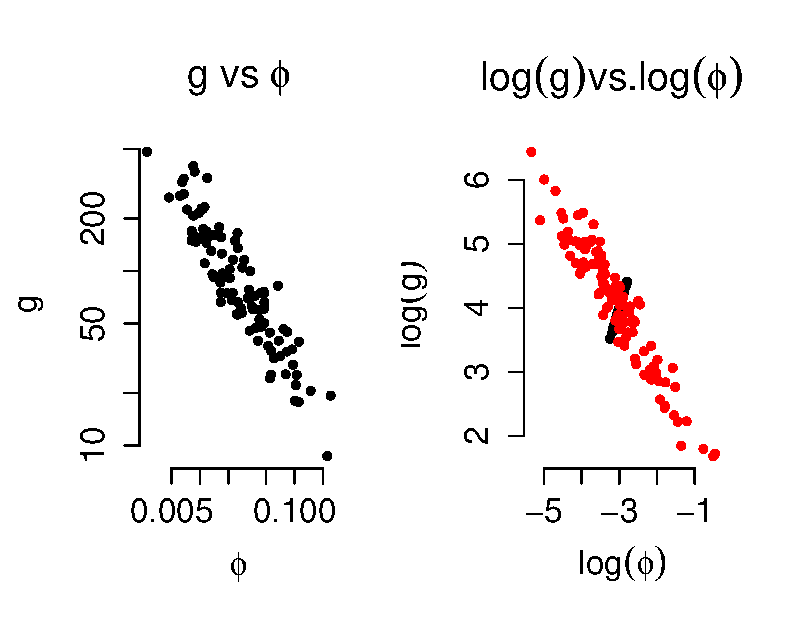
\includegraphics[scale=1]{g_vs_phi.eps}
\caption{Left: Plot of sensitivity $g$ against SEMPPR $\phi$ values for 106 genes in yeast data on $\log$ scale. Right: Plot of simulated data, black dots are from true values of $\phi$ and red dots are $\phi$ values with noise.}
\label{fig:gvsphi}
\end{figure}

\subsubsection{Confidence of estimates of optimal amino acids}
To get the confidence level of the estimates for optimal amino acid at each site with the maximizing approach, we found the smallest set of amino acids being optimal that cover more than 95\% of the total likelihood.
In Rokas's data there are about 9000 different site patterns at the 8 species.
For each of the 9000+ sites, the likelihood values achieved by assuming each amino acid as optimal is ordered decreasingly, therefore the likelihood under the max optimal amino acid is ranked the first.
Then the next amino acid is included in the optimal set of amino acids until the total likelihood exceeds 95\% of the total likelihood.
Figure \ref{fig:AAnum} shows the histogram of numbers of optimal amino acids in the set.
The mean value for all 9000+ patterns is 5.855, and mode is 6.
The case where there are more than 10 amino acids in the set rarely happened.
Figure \ref{fig:percentile} showed the density of percentages of total likelihood value covered by the optimal amino acid found with max rule only.
Mean percentage is 0.4749 and the peak of the density distribution is between 0.3 and 0.4. (How confident are we now??)

\begin{figure}[h]
\centering
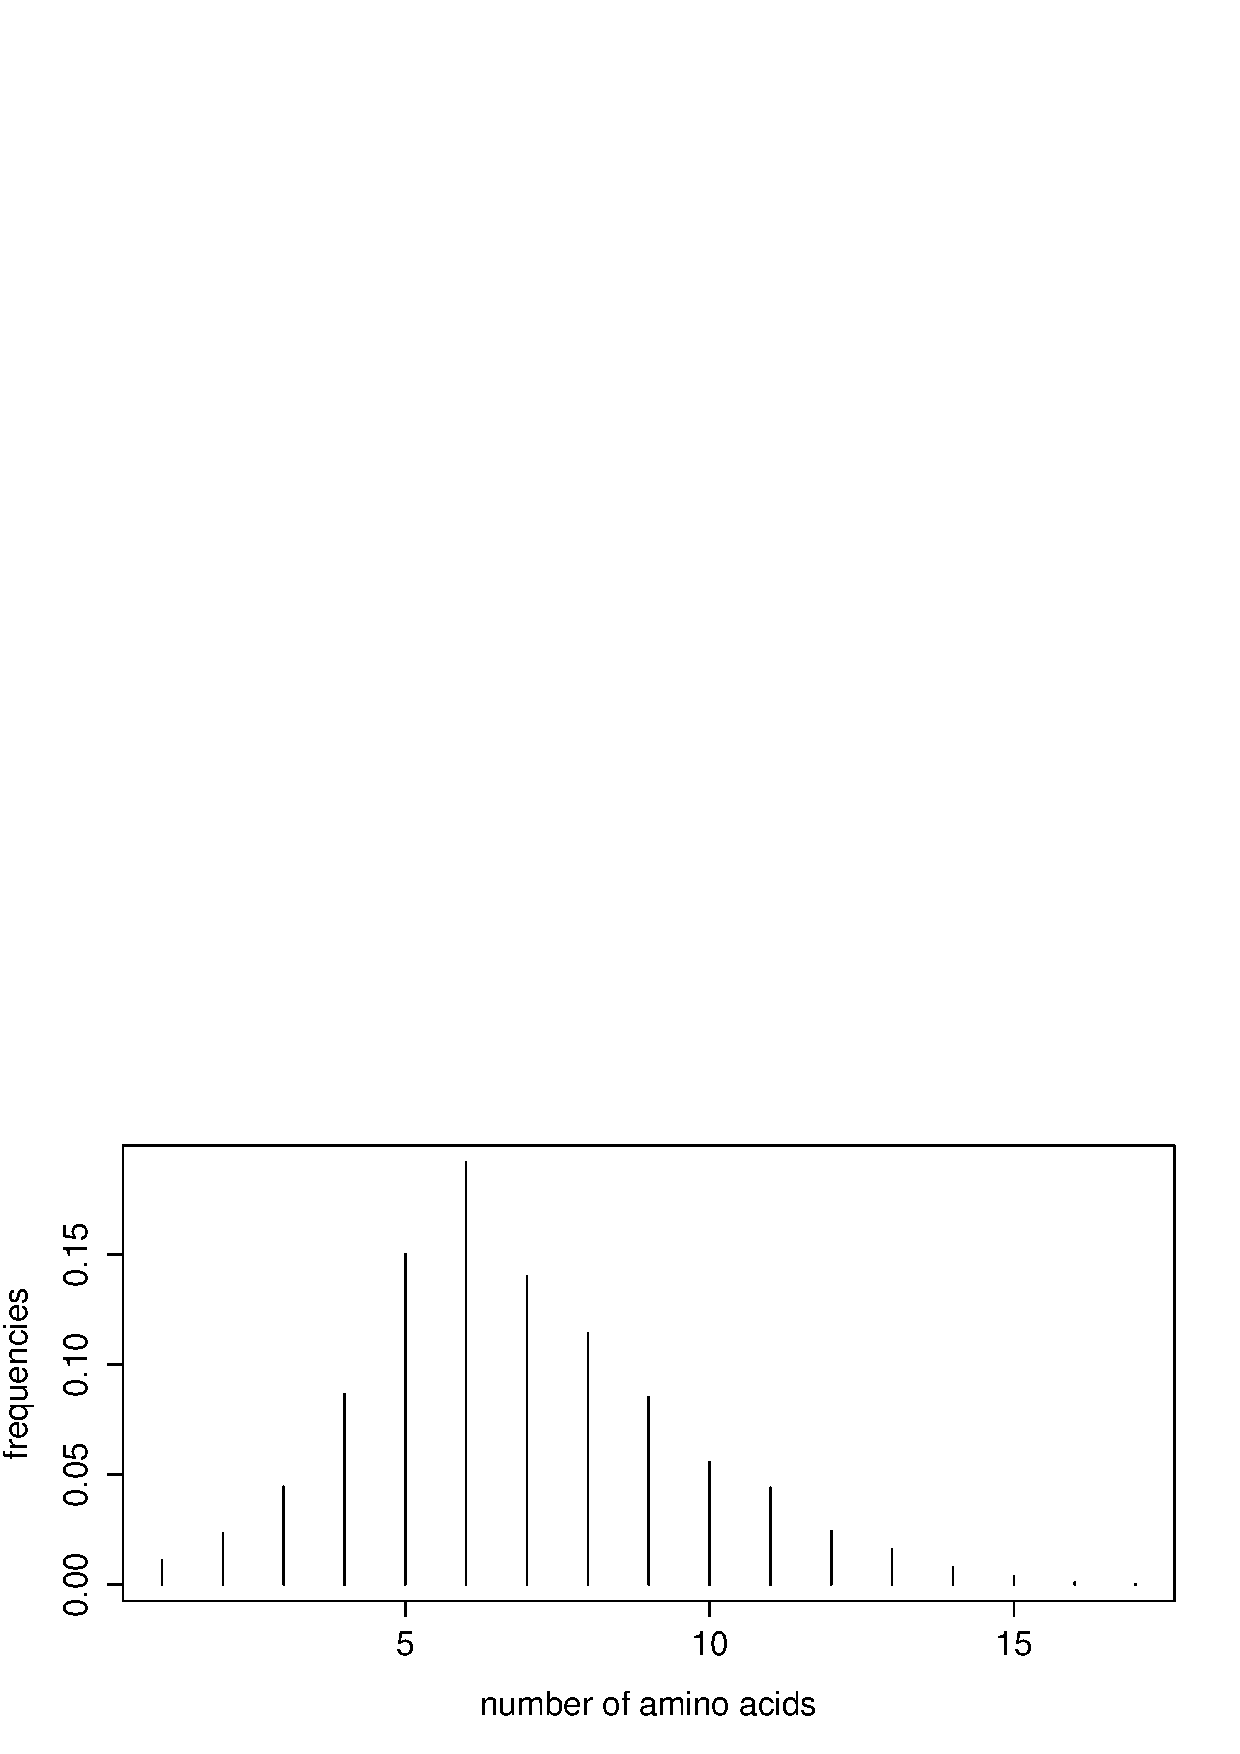
\includegraphics[width=\textwidth]{AAnum.pdf}
\caption{Histogram of the number of optimal amino acids together to cover at least 95\% of the total likelihood attained by all possible optimal amino acids.}
\label{fig:AAnum}
\end{figure}


\begin{figure}[h]
\centering
\includegraphics[width=\textwidth]{percentile.pdf}
\caption{Density plot of percentages of the likelihood achieved by the optimal amino acid found by max rule.}
\label{fig:percentile}
\end{figure}


%\subsubsection{Model accuracy}
%To assess model accuracy, we did simulations using the maximum likelihood estimates from Rokas et. al. 's data. (waiting on results)

\subsubsection{Simulated data vs. observed data}
We also evaluate the models by simulating data under models and comparing them with the observed data. 
First, a single taxon (Scas) is deleted from the Rokas's yeast gene tree, model parameters are estimated from the data on the remaining taxa. 
Then the ancestral sequence where the missing taxon is attached is estimated, where the probabilities of observing all 20 amino acids at each site are calculated. 
Then the deleted data is put back and the length of the truncated branch earlier is estimated using the parameters on the pruned tree. 
With the parameter values, the length of the missing branch, and the sequence at the start of the branch, we simulate the evolution of a gene's coding sequence from the reconstructed taxon to the deleted taxon from our analysis.
We then compare the simulated sequence at the deleted taxon with the real data. 
\begin{figure}[h]
\centering
\includegraphics[width=\textwidth]{simulation.png}
\label{fig:simulation}
\end{figure}
The results are shown in Figure \ref{fig:simulation}. 
On the left, each dot represents the proportion of amino acids that differ between the simulated and the observed sequence for a given gene. 
Our new model performed much better than the standard WAG model in matching sequences, especially for genes under high selection that are shown in brighter dots. 
On the right repeated simulations are plotted under our new model (red) and WAG model (blue) starting from the ancestral sequence estimated under the estimated sequences under the new model (upper lines) and WAG model (lower lines) for a single gene. 
The dotted line represents the functionality for the observed sequence.
When the ancestral sequences are estimated from WAG model, they have much lower fitnesses. 
If evolved under WAG model, the fitness does not improve much at the end of the branch.
On the other hand there is directional selection leading to an increase in fitness if the sequences evolve under the new model. 
When the ancestral sequences are estimated from the new model the fitness is significantly higher. 
And WAG simulation leads to a decrease in fitness while the fitness is maintained under simulation with the new model.
No matter how the ancestral sequences are obtained, the new model presents a better match to the observed data.
This realistic behavior shows that the new model is more adequate than the WAG model for Rokas's data. [I THINK WE SHOULD USE THE ACTUAL BEST MODEL UNDER PROTTEST, PLUS  AA BASED ON GY94 AND GTR CODON/NUCLEOTIDE MODELS]

\subsection{Result on insect data}
We also analyzed the model performance on the insect data used in \cite{McKenna2010}. This DNA sequence data comprised of approximately 13 kb of aligned data from 7 single-copy nuclear protein-coding genes: elongation factor-1$\alpha$, alanyl-tRNA synthetase (AATS), carbamoylphosphate synthase domain (CAD), 6-phosphogluconate dehydrogenase (PGD), sans fille (SNF), triosephosphate isomerase (TPI), and RNA polymerase II (RNA Pol II). The taxon sample was comprised of 34 insects, including 32 exemplars representing all orders of holometabolous insects, and two hemimetabolous insect outgroups.

\begin{table}[h]
\begin{center}
\begin{tabular}{l r c r r}
\hline
Model & $\Delta$AIC & $l$ & Tree length & Parameters \\
\hline
New+maj & 0.00 & -257790.10 &  10.43 & 41 \\
New+max & 48574.60 & -239735.40 & 11.73 & 42,383 \\
New+weights & 123688.60 & -319615.40 & 2.86 & 60 \\
LG+I+G+F & 81803.98 & -298699.09 &  & 34\\
LG+G+F & 81808.86 & -298702.53 & & 33 \\
\hline
\end{tabular}
\end{center}
\caption{Log-likelihood values and parameter estimates under empirical models and new model for the sequence with 42,342 amino acids}
\label{table:mle}
\end{table}